\section{مقدمه}
\subsection{برنامه‌ها}
در این پروژه می‌خواهیم که تاثیر
\lr{TLB shootdown}
بر روی انواع دیتابیس‌ها را مشاهده کنیم. دیتابیس‌هایی که ما انتخاب کردیم به شرح زیر هستند:
\begin{itemize}
	\item \lr{Redis}
	\item \lr{MySQL}
	\item \lr{Postgres}
	\item \lr{SQLite3}
	\item \lr{CockroachDB}
	\item \lr{Cassandra}
\end{itemize}
همچنین قرار است که در ادامه کمی نیز بر روی نرم‌افزار
\lr{nginx}
کار کنیم چرا که آن نیز در برخی از مواقع
\lr{bottleneck}
وب سرور‌ها است. همچنین در صورتی که بتوانیم می‌خواهیم که از
\lr{syscall}های
\link{https://en.wikipedia.org/wiki/Io_uring}{io\_uring}
برای تست نیز استفاده کنیم. یک
\lr{patch}
(\link{https://github.com/hakasenyang/openssl-patch/issues/21}{لینک})
برای کتابخانه‌های
\lr{nginx}
وجود دارد که به کمک آن می‌توانیم از توابع جدید
\lr{io\_uring}
که برای
\lr{async io}
نوشته شده‌اند استفاده کنیم. به کمک این توابع می‌توانیم عملکرد آن‌ها را با
\link{https://en.wikipedia.org/wiki/Epoll}{epoll}
مقایسه کنیم.

این آزمایش را در چندین محیط و نسخه‌ی کرنل انجام می‌دهیم.
\subsection{محیط‌ metal bare}
در این محیط صرفا ما صرفا بر روی لپتاپ‌های خود یک سیستم‌عامل
\lr{Ubuntu 20.04.6}
را بالا آوردیم و در آن برنامه‌های ذکر شده و کرنل‌های لینوکس را نصب کردیم. مشخصات دستگاه‌های هر یک از ما به شرح
زیر است:

\smalltitle{هیربد:}
\begin{latin}
\begin{itemize}
	\item Intel® Core™ i7-9750H Processor
	\item 16GB DDR3 RAM
	\item OS installed on HDD. 150 GB space.
	\item GTX 1650 Ti
	\item KVM virtualization enabled
\end{itemize}
\end{latin}
\smalltitle{هومان:}
\begin{latin}
\begin{itemize}
	\item Intel® Core™ i7-10750H Processor
	\item 12GB DDR4 RAM
	\item OS installed on HDD. 150 GB space.
	\item GTX 1650 Ti
	\item KVM virtualization enabled
\end{itemize}
\end{latin}

\subsection{محیط‌ virtual}
\smalltitle{نصب}\\
برای محیط مجازی ما تصمیم به استفاده از
\lr{KVM}
گرفتیم. برای راه‌اندازی آن در ابتدا باید پکیج‌های مورد نیاز از
\lr{apt}
را به کمک دستور زیر نصب کنیم:
\codebox{apt install qemu-kvm libvirt-daemon-system libvirt-clients bridge-utils virt-manager}
سپس به کمک دستورات زیر باید به کاربر جاری اجازه دهیم که از
\lr{KVM}
بتواند استفاده بکند.
\codebox{sudo adduser 'hirbod' libvirt\\sudo adduser 'hirbod' kvm}
سپس به کمک دستور
\codeword{systemctl status libvirtd}
می‌توان چک کرد که آیا
\lr{KVM}
فعال است یا خیر.
\begin{figure}[H]
    \centering
    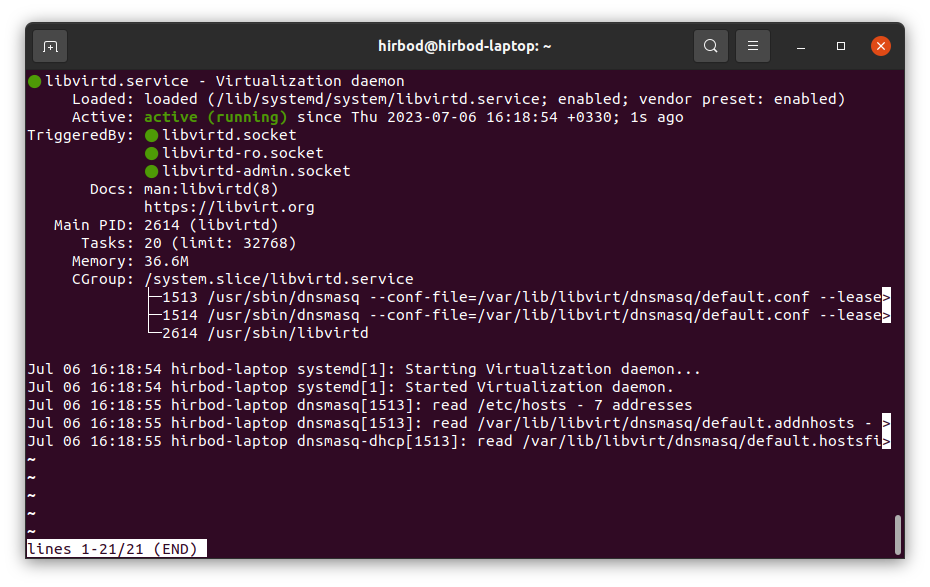
\includegraphics[scale=0.3]{pictures/intro/kvm.png}
    \caption{\lr{KVM service}}
    \label{fig:into:kvm}
\end{figure}
یک نکته‌ای که وجود دارد این است به صورت پیش‌فرض
\lr{KVM} از \link{https://en.wikipedia.org/wiki/Qcow}{qcow2}
استفاده می‌کند که یک نوع فایل
\lr{thin provisioned}
برای ذخیره سازی داده‌های یک ماشین مجازی هست. ولی از آنجا که کار ما
\lr{IO intensive}
است، بهتر است که از
\lr{thin provisioning}
استفاده نکنیم. به همین منظور باید دیسک مجازی را به حالت
\lr{raw}
در بیاوریم. برای این کار ما از
\link{https://easyengine.io/tutorials/kvm/convert-qcow2-to-raw-format/}{این}
مراحل استفاده کردیم. یعنی کافی است که در ابتدا دستور زیر را در ترمیال بزنیم که دیسک تبدیل به نسخه‌ی
\lr{raw}
شود.
\codebox{qemu-img convert vm.qcow2 vm.raw}
سپس به کمک دستور
\codeword{virsh edit vm1}
تنظیمات ماشین مجازی را می‌توان عوض کرد. کافی است که قسمت
\codeword{disk}
را پیدا کنیم و هم نوع آنرا از
\lr{qcow2} به \lr{raw}
و هم مسیر آنرا آپدیت کنیم.

\subsection{کامپایل کرنل}
در این آزمایش ما تصمیم گرفتیم که کرنل‌های
\lr{3.19.8}، \lr{4.19.284} و \lr{6.3.6}
استفاده کنیم. همچنین برای ورژن 5 از هر چیزی که بر روی سیستم بای دیفالت نصب بود استفاده می‌کردیم.
به عنوان مثال در نسخه‌ی
\lr{bare metal}
که در
\lr{Ubuntu desktop}
نصب شده است، از ورژن کرنل
\lr{5.15.73}
استفاده می‌کردیم و در ماشین‌های مجازی که از
\lr{Ubuntu server}
استفاده می‌کردند از نسخه‌های
\lr{5.4.150}
استفاده می‌کردیم.

برای شروع در ابتدا به کمک دستور زیر برنامه‌های مورد نیاز را دانلود می‌کنیم:
\codebox{apt install build-essential dwarves python3 libncurses-dev flex bison libssl-dev bc libelf-dev zstd gnupg2 wget curl git}
سپس سورس‌کد‌های لینوکس را از سایت
\link{https://kernel.org/}{kernel.org}
دانلود می‌کنیم و از حالت فشرده خارج می‌کنیم.

سپس باید کانفیگ کرنل را بسازیم. برای
\lr{safe}
بودن از خود کانفیگی که برای سیستم‌عامل فعلی است استفاده می‌کنیم. برای این کار صرفا از کامند زیر
استفاده می‌کنیم:
\codebox{cp /boot/config-\$(uname -r) .config}
این دستور کانفیگی که کرنل فعلی سیستم‌عامل با آن کامپایل شده است را به عنوان کانفیگی که ما می‌خواهیم
کرنل با آن کامپایل شود قرار می‌دهد.

سپس دستور
\lr{make menuconfig}
را می‌زنیم. این دستور یک منو برای کانفیگ کردن کرنل را به ما نشان می‌دهد. اما کار مهم تری که می‌کند این است که
سعی می‌کند که مشکلات فایل کانفیگی که داشتیم را برطرف بکند؛ دقت کنید که از آنجا که نسخه‌ی کرنلی که می‌خواهیم
کامپایل کنیم با نسخه‌ی کرنل سیستم‌عامل خیلی فرق دارد برای همین یک سری تنظیمات وجود دارد که در کانفیگ فایل نیست
یا برعکس. این دستور علاوه بر نشان دادن همه‌ی تنظیمات سعی می‌کند که مقادیر دیفالت قابل قبولی برای
این کانفیگ قرار دهد.

در نهایت به کمک دستور
\codeword{make -j 12}
می‌توان کرنل را کامپایل کرد که 12 تعداد هسته‌های
\lr{CPU}
است. بعد از کامپایل شدن به کمک دستور
\codeword{make modules\_install}
ماژول‌هایی که کامپایل شده است را نصب می‌کنیم و سپس در نهایت به کمک
\codeword{make install}
کرنل را به
\lr{GRUB}
اضافه می‌کنیم که بتوانیم آنرا
\lr{boot}
کنیم.

یکی از مشکلاتی که معمولا در کامپایل لینوکس پیش می‌آید یک
\lr{key chain}
برای امضا کردن ماژول‌هاست. برای اینکه به مشکلی سر کامپایل کردن بر نخوریم، صرفا کافی است که فایل
\codeword{.config}
را با یک
\lr{text editor}
باز کنیم و آپشن‌هایی که فایلی دارند که پسوند آن
\codeword{.pem}
است را حذف کنیم. من حدس میزنم که این ماژول‌ها با یک
\lr{private key}
مخصوص خود
\lr{Ubuntu sign}
شده‌اند که مشخصا در کامپیوتر ما موجود نیست.

هر یک از نسخه‌های کرنل قلقی برای راه اندازی خودشان داشتند که هر کدام از آن‌ها را در اینجا
ذکر می‌کنیم.

\smalltitle{\lr{3.19.8}}
\\\noindent
مشکلی که این نسخه‌ی کرنل داشت این بود که فوق العاده قدیمی هست و برای همین آخرین نسخه‌ی
\lr{GCC}
نمی‌تواند آنرا کامپایل کند! به همین جهت یک ایده‌ای که به ذهنم رسید این بود که لینوکس را در داکر
کامپایل کنم. به همین جهت داکر را نصب کردم و یک ایمیج نسخه‌ی
\lr{14.04}
بالا آوردم و در این کانتینر دقیقا همان کار‌های بالا را انجام دادم با این تفاوت که فایل
\codeword{.config}
را از
\lr{host}
به کانتینر آوردم و صرفا
\codeword{make}
زدم. سپس کل فولدری که در آن کامپایل را انجام دادم را به
\lr{host}
منتقل کردم و در
\lr{host}
دستورات نصب را زدم. با این کار این ورژن به درستی نصب شد ولی مشکلی که وجود داشت این بود که
بعد از بالا آمدن لپتاپ با این ورژن موس پد کار نمی‌کرد! این مشکل خیلی حادی نبود و صرفا یک موس
\lr{USB}
دار کار می‌کرد. از آنجا که این مشکل خیلی حادی نبود از آن چشم پوشی کردم. اما یک مشکل اساسی‌تر رخ داد؛
داکر به صورت کلی از کار افتاد! یعنی سرویس
\lr{dockerd}
دیگر استارت نمی‌شد. پس نمی‌توانستیم دیتابیس‌ها از داکر نصب کنیم بر روی این نسخه‌ی کرنل\dots

اما مشکل اصلی این نسخه‌ی کرنل بر روی ماشین مجازی بود. زمانی که این کرنل را برای ماشین مجازی کامپایل
و نصب کردیم، دیگر نمی‌توانستیم آنرا
\lr{boot}
کنیم. با توجه به لاگ‌هایی که وجود داشت،‌ سیستم‌عامل نمی‌توانست پارتیشن‌های دیسک اصلی را بشناسد برای همین در
حالت
\lr{recovery mode}
می‌رفت مانند شکل
\ref{fig:into:kernel:vm3}.
ما کار‌هایی زیادی مثل عوض کردن
\lr{fdisk}،‌
غیر فعال کردن
\lr{virtio} و
چک کردن اینکه آیا این ماژول فعال است انجام دادیم ولی با این حال نتوانستیم آنرا بوت کنیم.
\begin{figure}[H]
    \centering
    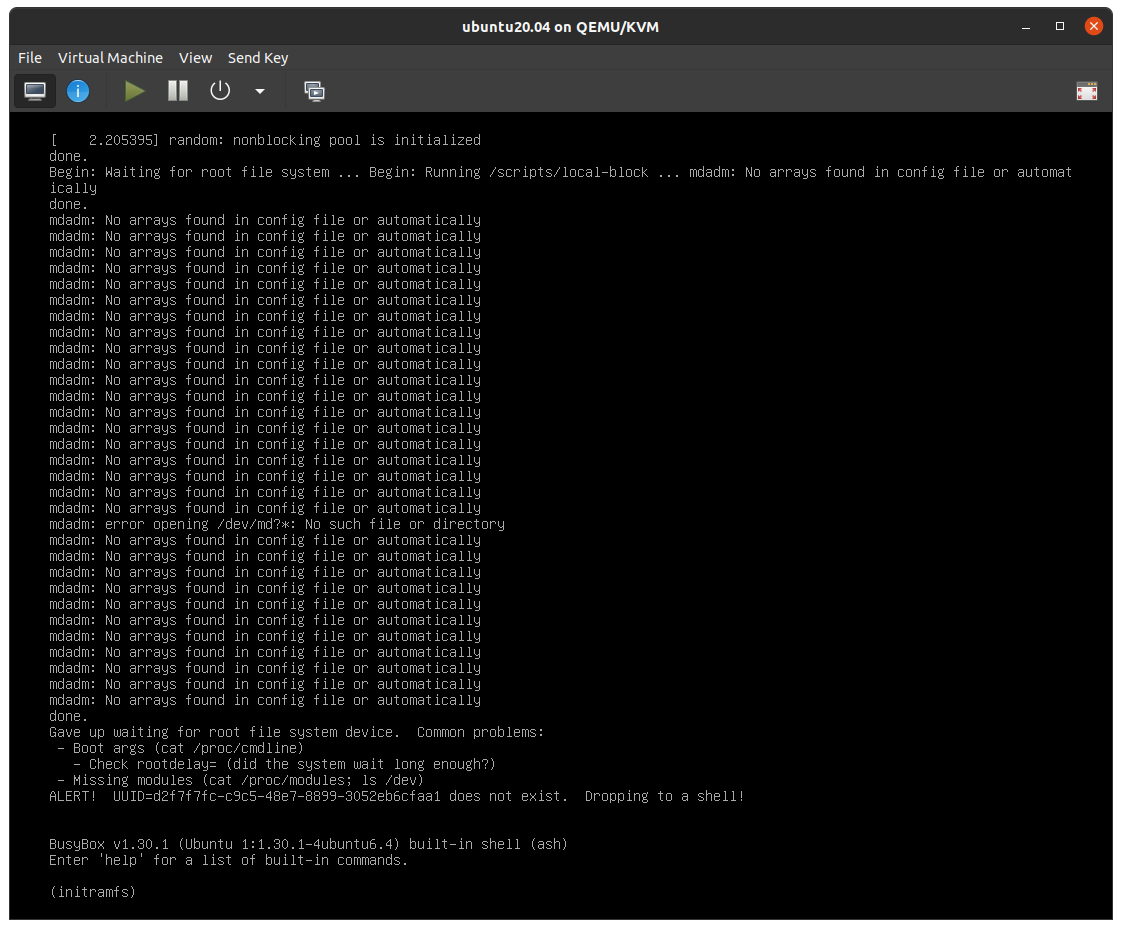
\includegraphics[scale=0.3]{pictures/intro/kvm-kernel-3.png}
    \caption{بوت نشدن ماشین مجازی در کرنل نسخه‌ی 3}
    \label{fig:into:kernel:vm3}
\end{figure}

\smalltitle{\lr{4.19.284}}
\\\noindent
این نسخه خیلی چالش خاصی نداشت و صرفا توانستیم آنرا با زدن دستورات بالا نصب کرد.
\\
\textbf{آپدیت}
\\
در این کرنل به یک مشکل همانند کرنل ۶.۳.۶ برخوردیم که خوب مشکل زیر بود 
\codebox{cannot stat 'arch/x86/crypto/aegis128-aesni.ko'}
احتمالا به دلیل مشکلات کلید کرنل است که با زدن دستور زیر درست شد.
\codebox{sed -ri '/CONFIG\_SYSTEM\_TRUSTED\_KEYS/s/=.+/=""/g' .config}
\\
\smalltitle{\lr{6.3.6}}
\\\noindent
کرنل نسخه‌ی 6 هم خیلی مشکلی نداشت صرفا با توجه به
\link{https://techviewleo.com/install-linux-kernel-6-on-ubuntu/}{این}
لینک باید دستور زیر را نیز اجرا می‌کردیم که کلید‌های امضا را غیر فعال کند:
\codebox{scripts/config --disable SYSTEM\_REVOCATION\_KEYS}

\smalltitle{\lr{Host To VM}}
\\\noindent
یکی دیگر از کار‌هایی که سعی کردیم بکنیم این بود که این نسخه‌های کامپایل شده‌ی کرنل را از محیط
\lr{bare metal}
به محیط مجازی ببریم. ولی متاسفانه نتوانستیم این کار را انجام دهیم. مشکلی که وجود داشت این بود که بعد از
دستورات نصب ماژول‌ها و نصب خود کرنل سیستم‌عامل به خاطر پیدا نکردن پارتیشن خودش بالا نمی‌آمد. با کمی سرچ به
\link{https://www.reddit.com/r/linuxquestions/comments/11xjdju/emergency_shell_after_update/}{این}
و
\link{https://askubuntu.com/q/15515/746382}{این}
سوال نیز رسیدیم ولی نتواسنیتم آنرا درست کنیم. نسخه‌ی قبلی کرنل به درستی لود می‌شد ولی نسخه‌ی جدید خیر.
این موضوع را هم با ورژن 3 و هم با ورژن 6 تست کردیم و در همه‌ی حالات به مشکل خوردیم. پس سعی کردیم که کرنل
را خودمان کامپایل کنیم.

\smalltitle{\lr{Perf}}
\\\noindent
یک موضوعی که باید به آن توجه کرد
\lr{perf}
است.
\lr{perf}
در هر نسخه‌ی لینوکس با نسخه‌ی دیگر متفاوت است. پس در نتیجه برای هر نسخه‌ی کرنلی که ما می‌خواهیم از آن استفاده
کنیم می‌بایستی
\lr{perf}
را نیز کامپایل کنیم. خوشبختانه
\lr{perf}
در کنار کرنل لینوکس قرار دارد و نصب آن ساده است. ما از
\link{https://scicoding.com/how-to-compile-perf-with-all-features-on/}{این}
راهنما استفاده کردیم و صرفا لازم بود که چیزی که داخل
\lr{tools/perf}
بود را
\codeword{make}
کنیم. با این کار فایل اجرایی
\lr{perf}
در همان پوشه ساخته می‌شد.

\smalltitle{\lr{Perf in VM}}
\\\noindent
یکی از مشکلاتی که می‌تواند به وجود آید این است در ماشین‌های مجازی
\lr{perf}
تمامی
\lr{event}ها را
\lr{<not supported>}
نشان دهد. این موضوع به دلیل تنظیمات
\lr{CPU KVM}
است. برای درست شدن آن کافی است مانند 
\link{https://access.redhat.com/documentation/en-us/red_hat_enterprise_linux/7/html/virtualization_tuning_and_optimization_guide/sect-virtualization_tuning_optimization_guide-monitoring_tools-vpmu}{این}
دستور العمل،‌ عمل کنیم. بدین منظور که دستور ادیت تنظیمات
\lr{VM}
را بزنیم و سپس خط مربوط به
\lr{CPU}
را به خط زیر تغییر دهیم:
\codebox{<cpu mode='host-passthrough'/>}
سپس با ری استارت کردن
\lr{VM}
مشکلات حل می‌شود.

\subsection{Pages Huge}
با توجه به تحقیقاتی که ما انجام دادیم،
\lr{huge pages}ها
نیازی نیست که در زمان کامپایل ورژن لینوکس ست شوند. بلکه کافی است که در
\codeword{/etc/sysctl.conf}
تنظیماتی را انجام دهیم. برای شروع دستور زیر را وارد می‌کنیم:
\codebox{\$ grep $\string^$Huge /proc/meminfo\\
HugePages\_Total:       0\\
HugePages\_Free:        0\\
HugePages\_Rsvd:        0\\
HugePages\_Surp:        0\\
Hugepagesize:       2048 kB\\
Hugetlb:               0 kB}
همان طور که مشاهده می‌شود
\lr{CPU}
ما از
\lr{huge pages}
پشتیبانی می‌کند و مقدار دیفالت آن صفحات دو مگابایتی است. برای فعال سازی
\lr{huge pages}
کافی است که خط زیر را به
\codeword{/etc/sysctl.conf}
اضافه کنیم:
\codebox{vm.nr\_hugepages = 200}
به عنوان مثال در اینجا ۲۰۰ صفحه ۲ مگابایتی را
\lr{allocate}
می‌کنیم. دقت کنید که این صفحات حالت 
\lr{demanding}
ندارند که تعداد آنها بتواند کم یا زیاد شود. بلکه باید از زمان
\lr{boot}
سیستم‌عامل تعداد آنها مشخص شده باشد و سیستم عامل دقیقا به همان اندازه صفحه درست می‌کند.
بعد از ست کردن این عدد سیستم را ری استارت می‌کنیم. من برای تست‌ها ۵۰۰ عدد یعنی برابر ۱ گیگابایت
را در نظر گرفتم.

بعد از ری‌استارت سیستم در صورتی که دوباره دستور فرق را بزنیم خروجی به صورت زیر است:
\codebox{\$ grep $\string^$Huge /proc/meminfo\\
HugePages\_Total:     500\\
HugePages\_Free:      500\\
HugePages\_Rsvd:        0\\
HugePages\_Surp:        0\\
Hugepagesize:       2048 kB\\
Hugetlb:         1024000 kB}
همان طور که مشخص است حال در حال استفاده از
\lr{huge pages}
هستیم. جالب است که اگر
\lr{htop}
را نیز نگاه کنیم می‌بینیم که حدودا یک گیگ بیشتر از حالت معمولی مموری در حال مصرف شدن است.
\begin{figure}[H]
    \centering
    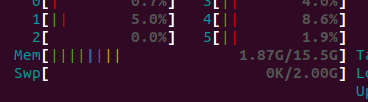
\includegraphics[scale=0.75]{pictures/intro/hugepages-htop.png}
    \caption{\lr{htop} بعد از فعال کردن \lr{huge pages}}
    \label{fig:into:hugepages:htop}
\end{figure}

% https://help.ubuntu.com/community/KVM%20-%20Using%20Hugepages